%% IEEE Journal of Biomedical and Health Informatics -- regular paper (single-blind).
%% Compile: pdflatex x2. Tables/figures read from ../empirical/{tables,figures} and ../integrated/.
\documentclass[journal]{IEEEtran}
\usepackage[T1]{fontenc}\usepackage[utf8]{inputenc}\usepackage{lmodern}
\usepackage{booktabs}\usepackage{graphicx}\usepackage{amsmath}\usepackage{array}\usepackage{xcolor}
\usepackage{adjustbox}\usepackage{tikz}\usetikzlibrary{arrows.meta,positioning,calc}\usepackage{enumitem}
\usepackage[hidelinks]{hyperref}\usepackage{url}
\definecolor{accent}{HTML}{8C2F1E}
\graphicspath{{../empirical/figures/}{../integrated/figures/}}
\makeatletter\def\input@path{{../empirical/}{../integrated/}{./}}\makeatother
% Generated tables open with \begin{table}[!htbp]. The redefinitions below take (and discard) that optional
% placement argument -- without the [1][] slot the string `[htbp]' is typeset as text above the table.
\let\origtable\table\let\endorigtable\endtable
\newcommand{\wideon}{\renewenvironment{table}[1][]{\begin{table*}[!t]}{\end{table*}}}
\newcommand{\wideoff}{\renewenvironment{table}[1][]{\begin{origtable}[!t]}{\end{origtable}}}
\begin{document}
\title{Leakage-Safe Evaluation of Machine-Learning Models for Mental-Health Prediction from Actigraphy: Protocol, Benchmark and Appraisal of Published Claims}
\author{Aminat~Abiola~Ajibola%
\thanks{A. A. Ajibola is with the College of Computer Science and Engineering, University of Hafr Al-Batin, Eastern Province, Kingdom of Saudi Arabia (e-mail: aajibola@uhb.edu.sa).}%
\thanks{Code, configurations, run manifests and generated tables: \url{https://github.com/rogerpanel/cv} (folder \texttt{mlmh-appraisal}, release v1.0.0-submission).}}
\markboth{IEEE Journal of Biomedical and Health Informatics}{Ajibola: Leakage-Safe Evaluation of ML Models for Mental-Health Prediction from Actigraphy}
\maketitle

\begin{abstract}
Machine-learning models that detect mental disorders from wrist actigraphy are benchmarked almost exclusively on three open cohorts, DEPRESJON, PSYKOSE and HYPERAKTIV, and reported accuracies have risen from the dataset authors' leave-one-patient-out 0.7 to above 0.9. We present a leakage-safe evaluation protocol for repeated-measures wearable data, apply it to these cohorts to establish reference baselines, and use it to explain the published claims. The protocol enforces participant-level splitting by a build-failing test, detects participants shared across cohorts from the activity series, fits all preprocessing inside folds, reports discrimination and calibration at window and participant level, and quantifies uncertainty with participant-level bootstrap intervals; every table is generated from run manifests. Nine experiments on 162 participants show that day-level cross-validation inflates AUROC by 0.02 to 0.17 relative to participant-level splitting, yields AUROC of 0.69 to 0.90 on labels randomly reassigned across participants, and that one day of activity re-identifies a participant with 27 to 40\% top-1 accuracy against 1 to 2\% chance: the inflation is memorisation. A state-of-the-art time-series method (ROCKET) reproduces the pattern. Frozen cross-cohort transfer loses up to 0.21 AUROC in one direction with calibration slopes of 0.27 to 0.63; honest slopes are 0.53 to 0.95 and are never reported in the literature. Of 28 published models on these cohorts, every accuracy above the honest band used or did not state a day-level unit, none reports calibration, and none validates on a second cohort. The protocol and baselines are released for future comparison.
\end{abstract}

\begin{IEEEkeywords}
Actigraphy, calibration, data leakage, depression, external validation, machine learning, reproducibility, schizophrenia, wearable sensing.
\end{IEEEkeywords}

\section{Introduction}
\IEEEPARstart{W}{rist} actigraphy counts movement once a minute for days at a time without any action by the wearer, and disturbed activity and circadian rhythm are among the best-replicated objective correlates of depression, psychosis and attention-deficit/hyperactivity disorder (ADHD). Three open datasets from Haukeland University Hospital and collaborating Norwegian sites, DEPRESJON \cite{garciaceja2018}, PSYKOSE \cite{jakobsen2020} and HYPERAKTIV \cite{hicks2021}, recorded with one device family and re-released in 2025 as the harmonised OBF-Psychiatric collection \cite{obf2025}, have become the default benchmarks for machine-learning (ML) detection of mental disorders from wearables. Reported accuracies on them have climbed from the dataset authors' leave-one-patient-out F1 of 0.73 \cite{garciaceja2018} to 0.85 to 0.96 for depression \cite{jmir2025,arxiv2303,zanella2019} and 0.92 to 0.94 for schizophrenia \cite{psykose_dl2024,psykose_bspc2024}.

Whether such numbers mean what they appear to mean depends on three aspects of evaluation. \emph{Which unit is held out}: each participant contributes many days, and days from one person resemble each other far more than anyone else's, so folds drawn over days (\emph{record-wise} splitting) let a model recognise the person rather than the disorder \cite{saeb2017,jmirai2026}. \emph{Whether the model is tested on a second population}: a frozen model applied to an independent cohort is the standard test of transfer and is rarely done; here it carries a trap, because PSYKOSE reuses DEPRESJON's 32 controls. \emph{Whether probabilities are calibrated}: a screening tool is used through its probabilities, and calibration is essentially never reported for wearable-based models \cite{vancalster2019}. The PROBAST+AI risk-of-bias tool \cite{moons2025} and the TRIPOD+AI reporting statement \cite{collins2024} make all three explicit requirements; an appraisal of psychiatric prediction models found calibration reported in 22\% and adequate internal validation in 11\% \cite{meehan2022}.

This paper makes four contributions.
\begin{enumerate}[nosep,leftmargin=*]
\item \textbf{A leakage-safe evaluation protocol} for repeated-measures wearable data, implemented as a tested, public codebase: participant-level splitting enforced by a build-failing test, cross-cohort participant overlap detected from the data, preprocessing inside folds, window- and participant-level metrics with calibration, participant-level bootstrap intervals, and run manifests from which every table is generated (Section~\ref{sec:protocol}).
\item \textbf{Reference baselines} on the three cohorts and OBF-Psychiatric under that protocol, for fixed tabular models, a 1D-CNN and ROCKET, with cross-cohort transfer, calibration, sex strata, transdiagnostic and five-class tasks, and ablations (Sections~\ref{sec:exp}--\ref{sec:results}).
\item \textbf{A mechanistic account of the inflation}: a label-permutation test showing that record-wise splitting scores memorisation on labels with no disorder signal, and a re-identification test quantifying the participant fingerprint in one day of activity (Section~\ref{sec:mech}).
\item \textbf{An appraisal of the 28 published models} on these cohorts against the measured honest and leaky bands, using PROBAST+AI and TRIPOD+AI criteria (Section~\ref{sec:claims}).
\end{enumerate}

\section{Data}\label{sec:data}
\wideon\input{tables/cohort_characteristics}\wideoff
DEPRESJON \cite{garciaceja2018}: 23 patients with unipolar or bipolar depression (MADRS median 24) and 32 healthy controls. PSYKOSE \cite{jakobsen2020}: 22 inpatients with schizophrenia (BPRS median 51) and the same 32 controls. HYPERAKTIV \cite{hicks2021}: adults referred for ADHD assessment, of whom 45 with ADHD and 40 clinical controls (psychiatric outpatients without ADHD) have activity recordings, read from OBF-Psychiatric \cite{obf2025}. All were recorded with an Actiwatch at one-minute resolution (Table~\ref{tab:cohorts}). Hashing each participant's activity series confirmed that the 32 PSYKOSE control recordings are byte-identical to the DEPRESJON control recordings and that OBF-Psychiatric contains each of the 162 participants exactly once. The analysis unit is one calendar day with at least 80\% valid minutes; partial first and last days were dropped, giving 1{,}034, 1{,}021 and 502 days (1{,}818 unique). Labels are participant-level diagnostic groups. Twenty-eight features per day (Supplementary Table S2) cover distributional statistics, day/night contrasts, non-parametric circadian measures (M10, L5, relative amplitude, intradaily variability, M10-onset phase), autocorrelation, spectral summaries, rest/activity transitions and missingness; no demographic variable is used. The $\log(1+x)$ 1440-minute series is used by the 1D-CNN and ROCKET.

\section{Evaluation protocol}\label{sec:protocol}
% Figure 1: architectural framework of the study (TikZ). Included by manuscript_AB.tex.
\begin{figure*}[!t]\centering
\resizebox{\textwidth}{!}{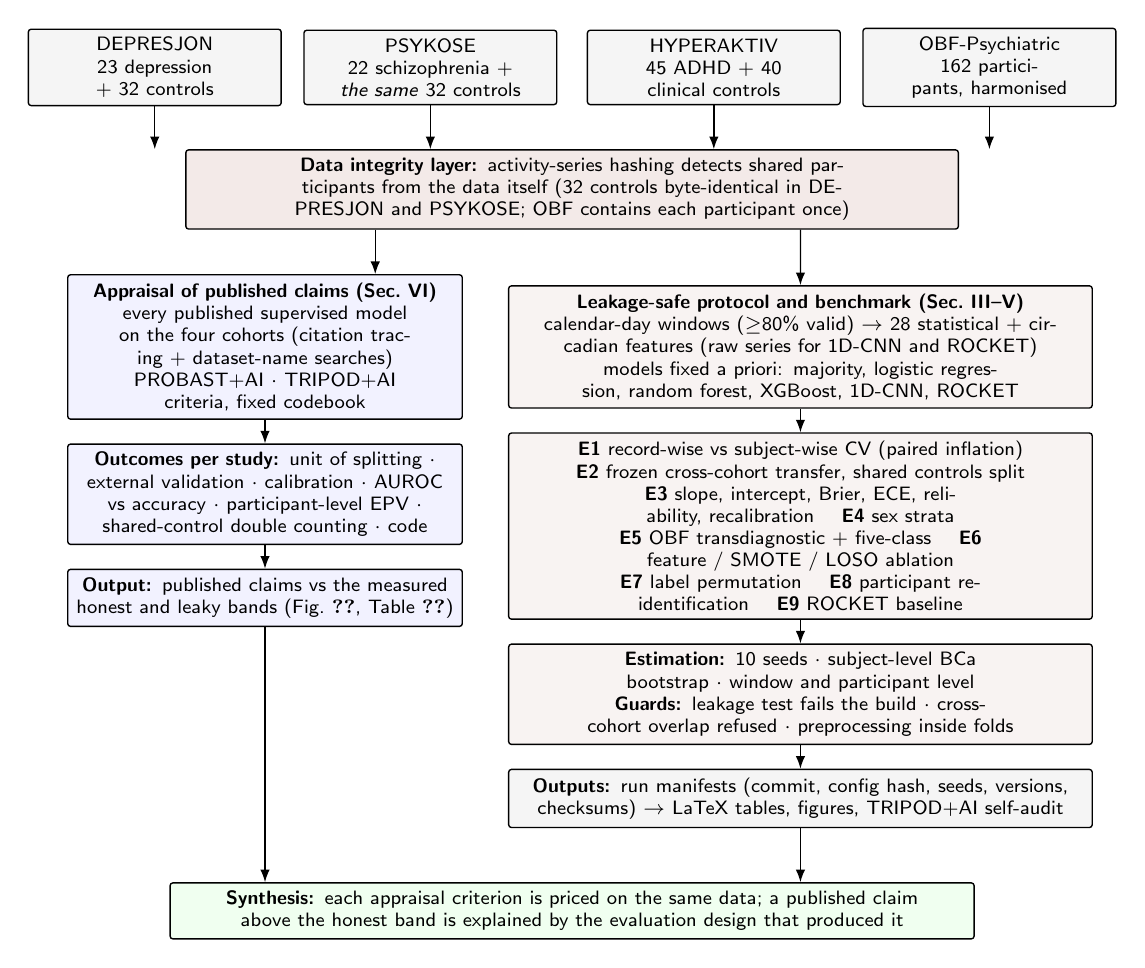
\begin{tikzpicture}[x=1cm,y=1cm,
  font=\sffamily\scriptsize,
  box/.style={draw, rounded corners=1pt, align=center, inner sep=3pt, minimum height=7mm, fill=white, line width=0.5pt},
  data/.style={box, fill=gray!8, text width=30mm},
  p1/.style={box, fill=blue!5, text width=48mm},
  p2/.style={box, fill=accent!6, text width=72mm},
  arr/.style={-{Latex[length=1.6mm]}, line width=0.5pt}]
% ----- data layer
\node[data] (dep) at (-5.3,0) {DEPRESJON\\23 depression + 32 controls};
\node[data] (psy) at (-1.8,0) {PSYKOSE\\22 schizophrenia + \emph{the same} 32 controls};
\node[data] (hyp) at (1.8,0) {HYPERAKTIV\\45 ADHD + 40 clinical controls};
\node[data] (obf) at (5.3,0) {OBF-Psychiatric\\162 participants, harmonised};
\node[box, fill=accent!10, text width=96mm] (hash) at (0,-1.55) {\textbf{Data integrity layer:} activity-series hashing detects shared participants from the data itself (32 controls byte-identical in DEPRESJON and PSYKOSE; OBF contains each participant once)};
\foreach \n in {dep,psy,hyp,obf} \draw[arr] (\n.south) -- (\n.south|-hash.north);
% ----- Part I (left column)
\node[p1] (p1a) at (-3.9,-3.55) {\textbf{Appraisal of published claims (Sec.~VI)}\\every published supervised model on the four cohorts (citation tracing + dataset-name searches)\\PROBAST+AI $\cdot$ TRIPOD+AI criteria, fixed codebook};
\node[p1, below=3mm of p1a] (p1b) {\textbf{Outcomes per study:} unit of splitting $\cdot$ external validation $\cdot$ calibration $\cdot$ AUROC vs accuracy $\cdot$ participant-level EPV $\cdot$ shared-control double counting $\cdot$ code};
\node[p1, below=3mm of p1b] (p1c) {\textbf{Output:} published claims vs the measured honest and leaky bands (Fig.~\ref{fig:part1}, Table~\ref{tab:sota})};
% ----- Part II (right column)
\node[p2] (p2a) at (2.9,-3.55) {\textbf{Leakage-safe protocol and benchmark (Sec.~III--V)}\\calendar-day windows ($\geq$80\% valid) $\rightarrow$ 28 statistical + circadian features (raw series for 1D-CNN and ROCKET)\\models fixed a priori: majority, logistic regression, random forest, XGBoost, 1D-CNN, ROCKET};
\node[p2, below=3mm of p2a] (p2b) {\textbf{E1} record-wise vs subject-wise CV (paired inflation) \quad \textbf{E2} frozen cross-cohort transfer, shared controls split\\\textbf{E3} slope, intercept, Brier, ECE, reliability, recalibration \quad \textbf{E4} sex strata\\\textbf{E5} OBF transdiagnostic + five-class \quad \textbf{E6} feature / SMOTE / LOSO ablation\\\textbf{E7} label permutation \quad \textbf{E8} participant re-identification \quad \textbf{E9} ROCKET baseline};
\node[p2, below=3mm of p2b] (p2c) {\textbf{Estimation:} 10 seeds $\cdot$ subject-level BCa bootstrap $\cdot$ window and participant level\\\textbf{Guards:} leakage test fails the build $\cdot$ cross-cohort overlap refused $\cdot$ preprocessing inside folds};
\node[p2, below=3mm of p2c, fill=gray!8] (p2d) {\textbf{Outputs:} run manifests (commit, config hash, seeds, versions, checksums) $\rightarrow$ LaTeX tables, figures, TRIPOD+AI self-audit};
\draw[arr] ([xshift=-2.5cm]hash.south) -- ([xshift=-2.5cm]hash.south|-p1a.north);
\draw[arr] ([xshift=2.9cm]hash.south) -- (p2a.north);
\draw[arr] (p1a) -- (p1b); \draw[arr] (p1b) -- (p1c);
\draw[arr] (p2a) -- (p2b); \draw[arr] (p2b) -- (p2c); \draw[arr] (p2c) -- (p2d);
% ----- synthesis
\node[box, fill=green!6, text width=100mm] (syn) at ($(p2d.south)+(-2.9,-1.05)$) {\textbf{Synthesis:} each appraisal criterion is priced on the same data; a published claim above the honest band is explained by the evaluation design that produced it};
\draw[arr] (p1c.south) -- (p1c.south|-syn.north);
\draw[arr] (p2d.south) -- (p2d.south|-syn.north);
\end{tikzpicture}}
\caption{Architecture of the study. Four open actigraphy cohorts pass through a data-level integrity check (participant hashing) into the leakage-safe protocol and benchmark (Sections III to V) and the appraisal of published claims (Section VI); the synthesis maps every appraisal criterion to a measured cost.}\label{fig:framework}
\end{figure*}

Figure~\ref{fig:framework} shows the design. Four principles govern it.

\subsubsection{Participant is the unit of inference} A \emph{subject-wise} splitter (stratified group $k$-fold) never places a participant on both sides of a fold; a \emph{record-wise} splitter (stratified $k$-fold over days) exists only where its optimism is the object of study. An automated test fails the build if any other configuration requests it, and the cross-validation runner asserts fold disjointness at run time. Cross-cohort runs refuse any pair with a participant on both sides, by identifier or by activity-series hash. Bootstrap resampling draws participants, with all their days, never days.

\subsubsection{Models fixed a priori} Majority-class baseline; $L_2$ logistic regression ($C=1$, class-balanced); random forest (500 trees, minimum leaf 2, balanced subsampling); XGBoost (300 rounds, depth 3, learning rate 0.05, subsampling 0.8); a three-block 1D-CNN on the raw series (30 fixed epochs, class-weighted loss, no early stopping on the test fold); and ROCKET \cite{dempster2020} with 500 random kernels and a logistic head. Hyper-parameters were not tuned, so that a difference between two arms is a difference in evaluation design. Imputation and standardisation are fitted on training folds only inside an \texttt{imblearn} pipeline.

\subsubsection{Both discrimination and calibration, at both levels} AUROC (primary), accuracy, balanced accuracy, macro-F1, MCC, AUPRC; Brier score, calibration slope and intercept \cite{vancalster2019}, expected calibration error (ECE, ten bins) and reliability curves; all at \emph{window} level (the unit most papers report) and at \emph{participant} level (mean probability per participant, the unit a screening decision uses).

\subsubsection{Traceability} Ten seeds govern fold assignment and model randomness. Point estimates are computed on seed-averaged out-of-fold predictions; 95\% intervals are bias-corrected and accelerated bootstrap intervals from 1{,}000 participant resamples with a leave-one-participant-out jackknife. Every run writes a manifest (commit, configuration hash, seeds, package versions, dataset checksums) and every table in this paper is generated from the manifests by the released code.

\section{Experiments}\label{sec:exp}
\textbf{E1 leaky splitting}: five-fold CV under subject-wise and record-wise splitters on identical data and seeds; the estimand is the paired AUROC difference bootstrapped over the same participants. \textbf{E7 label permutation}: diagnostic labels randomly reassigned across participants (five permutations), then E1 repeated; an honest estimate must be 0.5. \textbf{E8 re-identification}: a multiclass classifier predicting \emph{which participant} a day belongs to, day-level stratified folds (inherent to the task), top-1 and top-5 accuracy against $1/N$. \textbf{E9 ROCKET}: E1 with the ROCKET baseline. \textbf{E2 external validation}: model fitted on all of cohort A, applied frozen to cohort B, against subject-wise CV on A; shared controls assigned at random to one cohort (16 each); DEPRESJON$\rightarrow$HYPERAKTIV is a deliberate label-shift control. \textbf{E3 calibration}: all E1 (subject-wise) and E2 models, plus logistic recalibration fitted on the training cohort's out-of-fold predictions and applied externally. \textbf{E5 OBF-Psychiatric}: any-psychiatric-versus-control and five-class tasks under both splitters. \textbf{E6 ablation}: feature groups dropped or used alone, SMOTE inside folds, leave-one-subject-out. \textbf{E4 sex strata} is reported in the supplement.

\section{Results}\label{sec:results}
\subsection{E1: leakage inflation}
\wideon% Auto-generated by mlmh.reporting.tables -- do not edit by hand.
\begin{table}[!htbp]
\centering
\caption{E1: discrimination under subject-wise versus record-wise cross-validation. Cells give the estimate on seed-averaged out-of-fold predictions with subject-level BCa 95\% bootstrap intervals; inflation is the paired record-wise minus subject-wise difference.}
\label{tab:e1}
\footnotesize
\begin{adjustbox}{max width=\linewidth}
\begin{tabular}{llllllll}
\toprule
Cohort & Model & Window AUROC subject-wise & Window AUROC record-wise & Window inflation & Subject AUROC subject-wise & Subject AUROC record-wise & Subject inflation \\
\midrule
depresjon & Majority class & 0.465 [0.292, 0.653] & 0.491 [0.459, 0.528] & 0.026 [-0.147, 0.218] & 0.423 [0.300, 0.551] & 0.427 [0.295, 0.555] & 0.001 [-0.191, 0.202] \\
depresjon & Logistic regression & 0.779 [0.675, 0.861] & 0.845 [0.781, 0.896] & 0.065 [0.024, 0.122] & 0.899 [0.822, 0.969] & 0.965 [0.927, 0.990] & 0.065 [0.011, 0.109] \\
depresjon & Random forest & 0.770 [0.681, 0.848] & 0.877 [0.823, 0.923] & 0.107 [0.058, 0.168] & 0.883 [0.812, 0.948] & 0.977 [0.949, 1.000] & 0.094 [0.041, 0.146] \\
depresjon & XGBoost & 0.764 [0.675, 0.842] & 0.878 [0.830, 0.918] & 0.114 [0.060, 0.181] & 0.874 [0.795, 0.947] & 0.985 [0.964, 1.000] & 0.111 [0.040, 0.175] \\
psykose & Majority class & 0.437 [0.267, 0.632] & 0.500 [0.470, 0.535] & 0.062 [-0.113, 0.241] & 0.419 [0.278, 0.557] & 0.462 [0.331, 0.593] & 0.043 [-0.148, 0.227] \\
psykose & Logistic regression & 0.907 [0.820, 0.942] & 0.927 [0.875, 0.955] & 0.020 [0.006, 0.041] & 0.974 [0.943, 1.000] & 0.994 [0.983, 1.000] & 0.020 [0.000, 0.043] \\
psykose & Random forest & 0.893 [0.798, 0.934] & 0.937 [0.890, 0.962] & 0.044 [0.017, 0.080] & 0.956 [0.913, 0.997] & 0.994 [0.983, 1.000] & 0.038 [0.000, 0.074] \\
psykose & XGBoost & 0.903 [0.810, 0.941] & 0.945 [0.907, 0.969] & 0.042 [0.016, 0.078] & 0.969 [0.935, 1.000] & 0.997 [0.991, 1.000] & 0.028 [0.000, 0.059] \\
hyperaktiv & Majority class & 0.493 [0.355, 0.628] & 0.483 [0.433, 0.533] & -0.010 [-0.170, 0.148] & 0.497 [0.398, 0.597] & 0.443 [0.349, 0.540] & -0.054 [-0.203, 0.106] \\
hyperaktiv & Logistic regression & 0.449 [0.360, 0.535] & 0.579 [0.486, 0.661] & 0.130 [0.095, 0.167] & 0.424 [0.328, 0.519] & 0.601 [0.502, 0.695] & 0.177 [0.131, 0.221] \\
hyperaktiv & Random forest & 0.443 [0.361, 0.534] & 0.612 [0.526, 0.692] & 0.169 [0.135, 0.206] & 0.424 [0.333, 0.518] & 0.641 [0.550, 0.722] & 0.217 [0.177, 0.257] \\
hyperaktiv & XGBoost & 0.442 [0.360, 0.524] & 0.593 [0.518, 0.664] & 0.151 [0.116, 0.186] & 0.438 [0.337, 0.530] & 0.652 [0.555, 0.732] & 0.214 [0.173, 0.261] \\
\bottomrule
\end{tabular}
\end{adjustbox}
\end{table}
\wideoff
\wideon\input{tables/e1_auroc_inflation_subject}\wideoff
\begin{figure*}[!t]\centering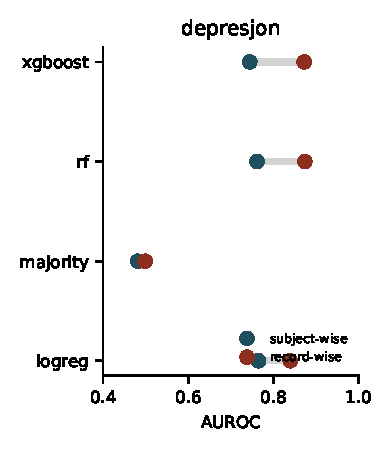
\includegraphics[width=\textwidth]{e1_inflation_auroc.pdf}
\caption{E1. Window-level AUROC under subject-wise (dark) and record-wise (red) five-fold cross-validation; the grey bar is the leakage inflation.}\label{fig:e1}\end{figure*}
Record-wise splitting raised AUROC for every informative model in every cohort at both levels (Tables~\ref{tab:e1} and~\ref{tab:e1subj}, Fig.~\ref{fig:e1}). On DEPRESJON, XGBoost rose from 0.764 (95\% CI 0.675 to 0.842) to 0.878 (0.830 to 0.918), a paired inflation of 0.114 (0.060 to 0.181); at participant level the honest 0.874 became 0.985. On PSYKOSE, where honest discrimination is already 0.893 to 0.907, inflation was 0.020 to 0.044 with participant-level leaky estimates of 0.994 to 0.997. On HYPERAKTIV the honest estimate was at or below chance for every model (0.442 to 0.449; participant level 0.424 to 0.438), yet record-wise splitting produced 0.579 to 0.612 and 0.601 to 0.652 respectively, an inflation of 0.130 to 0.169: leakage manufactured a signal. Logistic regression inflated least and the tree ensembles most in every cohort. The 1D-CNN did not exceed the feature models under honest splitting (0.696, 0.849, 0.459), was unstable across seeds, and its participant-level estimate rose from 0.738 to 0.912 on DEPRESJON under record-wise splitting (Supplementary Table S6).

\subsection{Mechanism: permutation, re-identification, ROCKET}\label{sec:mech}
\wideon% placeholder until E7 completes
\wideoff
With diagnostic labels randomly reassigned across participants (5 permutations; each participant keeps one label, but which one is random), no disorder signal remains and an honest estimate must sit at 0.5 (Table~\ref{tab:e7}). On DEPRESJON, subject-wise AUROC on permuted labels was 0.508 (logistic regression) and 0.517 (XGBoost), whereas record-wise AUROC was 0.646 (range over permutations 0.616 to 0.689) and 0.744 (0.721 to 0.768), reaching 0.740 and 0.898 at participant level. On PSYKOSE, subject-wise AUROC on permuted labels was 0.525 (logistic regression) and 0.506 (XGBoost), whereas record-wise AUROC was 0.638 (range over permutations 0.554 to 0.714) and 0.733 (0.701 to 0.799), reaching 0.719 and 0.895 at participant level. On HYPERAKTIV, subject-wise AUROC on permuted labels was 0.528 (logistic regression) and 0.533 (XGBoost), whereas record-wise AUROC was 0.621 (range over permutations 0.591 to 0.633) and 0.671 (0.641 to 0.703), reaching 0.666 and 0.753 at participant level. Under record-wise splitting the models therefore achieved discrimination comparable to the \emph{genuine} subject-wise results of E1 on labels that carry no information about the disorder at all: the design measures the model's ability to recognise a participant from other days of the same participant, and nothing else. The effect was larger for XGBoost than for logistic regression in every cohort, consistent with the E1 ordering.

% Auto-generated by mlmh.reporting.tables -- do not edit by hand.
\begin{table}[!htbp]
\centering
\caption{E8: participant re-identification from a single day of activity features (day-level stratified five-fold CV, three seeds). Top-1 accuracy far above chance quantifies the participant fingerprint that record-wise splitting exploits.}
\label{tab:e8}
\footnotesize
\begin{adjustbox}{max width=\linewidth}
\begin{tabular}{llccc}
\toprule
Cohort & Model & Participants (days) & Chance & Top-1 accuracy (SD) & Top-5 accuracy \\
\midrule
depresjon & Logistic regression & 55 (1034) & 0.018 & 0.330 (0.020) & 0.645 \\
depresjon & Random forest & 55 (1034) & 0.018 & 0.388 (0.031) & 0.718 \\
psykose & Logistic regression & 54 (1021) & 0.019 & 0.334 (0.029) & 0.651 \\
psykose & Random forest & 54 (1021) & 0.019 & 0.397 (0.043) & 0.721 \\
hyperaktiv & Logistic regression & 80 (490) & 0.013 & 0.271 (0.043) & 0.561 \\
hyperaktiv & Random forest & 80 (490) & 0.013 & 0.265 (0.030) & 0.572 \\
\bottomrule
\end{tabular}
\end{adjustbox}
\end{table}

A classifier trained to name the participant from one day of the same 28 features (Table~\ref{tab:e8}) identified the correct person, among 55, 54 and 80 candidates, with top-1 accuracy of 0.39, 0.40 and 0.26 (random forest) against chance levels of 0.02, 0.02 and 0.01, and placed the correct person in its top five in 0.72, 0.72 and 0.57 of days. One day of activity is thus a strong participant fingerprint, which is the resource that record-wise splitting hands to the model.

\wideon% Auto-generated by mlmh.reporting.tables -- do not edit by hand.
\begin{table}[!htbp]
\centering
\caption{E9: ROCKET time-series baseline (500 random convolutional kernels on the raw 1440-minute series, logistic head) under subject-wise and record-wise five-fold CV; window level, subject-level BCa intervals.}
\label{tab:e9}
\footnotesize
\begin{adjustbox}{max width=\linewidth}
\begin{tabular}{lccccc}
\toprule
Cohort & AUROC subject-wise & AUROC record-wise & Inflation (paired) & Participant AUROC (subj./rec.) & Cal. slope (subj.) \\
\midrule
depresjon & 0.717 [0.624, 0.799] & 0.831 [0.769, 0.871] & 0.114 [0.066, 0.167] & 0.857 / 0.976 & 0.36 \\
psykose & 0.865 [0.749, 0.908] & 0.905 [0.817, 0.935] & 0.040 [0.021, 0.068] & 0.949 / 0.980 & 0.67 \\
hyperaktiv & 0.506 [0.436, 0.571] & 0.575 [0.505, 0.627] & 0.069 [0.041, 0.092] & 0.535 / 0.657 & 0.00 \\
\bottomrule
\end{tabular}
\end{adjustbox}
\end{table}
\wideoff
To test whether the feature-based models understate the attainable ceiling, ROCKET \cite{dempster2020}, a state-of-the-art time-series method that applies 500 random convolutional kernels to the raw 1440-minute series and fits a regularised logistic head on the resulting 1{,}000 features, was evaluated under both designs (Table~\ref{tab:e9}). Its subject-wise AUROC was 0.717 (95\% CI 0.624 to 0.799) on DEPRESJON, 0.865 on PSYKOSE and 0.506 on HYPERAKTIV, below the feature-based models in every cohort, and record-wise splitting inflated it by 0.114 (0.066 to 0.167), 0.040 (0.021 to 0.068) and 0.069 (0.041 to 0.092), with participant-level leaky estimates of 0.976, 0.980 and 0.657. Its calibration slopes under honest splitting were 0.36, 0.67 and 0.00. A stronger learner therefore did not raise the honest ceiling; it reproduced the same inflation.


\subsection{E2: external validation}
\wideon% Auto-generated by mlmh -- do not edit by hand.
\begin{table}[!htbp]
\centering
\caption{E2: internal (subject-wise CV on the training cohort) versus external (unchanged model applied to the second cohort) performance. Window-level estimates, mean over seeds, subject-level BCa 95\% intervals. EPV = minority-class subjects per candidate predictor in the training cohort.}
\label{tab:e2}
\footnotesize
\begin{adjustbox}{max width=\linewidth}
\begin{tabular}{llllllllll}
\toprule
Train $\rightarrow$ Test & Model & EPV & Internal AUROC & External AUROC & $\Delta$ & Int. slope & Ext. slope & Ext. intercept & Ext. Brier \\
\midrule
depresjon $\rightarrow$ psykose & Majority class & 0.6 & 0.475 [0.224, 0.662] & 0.500 [0.500, 0.500] & +0.025 & -4.16 & 0.00 & -0.02 & 0.250 \\
depresjon $\rightarrow$ psykose & Logistic regression & 0.6 & 0.790 [0.701, 0.871] & 0.779 [0.676, 0.847] & -0.011 & 0.66 & 0.50 & 0.06 & 0.193 \\
depresjon $\rightarrow$ psykose & Random forest & 0.6 & 0.730 [0.607, 0.837] & 0.775 [0.688, 0.846] & +0.045 & 0.58 & 0.80 & -0.02 & 0.193 \\
depresjon $\rightarrow$ psykose & XGBoost & 0.6 & 0.716 [0.608, 0.825] & 0.768 [0.678, 0.835] & +0.051 & 0.34 & 0.55 & -0.01 & 0.204 \\
psykose $\rightarrow$ depresjon & Majority class & 0.6 & 0.463 [0.206, 0.601] & 0.500 [0.500, 0.500] & +0.037 & -4.07 & 0.00 & 0.06 & 0.250 \\
psykose $\rightarrow$ depresjon & Logistic regression & 0.6 & 0.881 [0.790, 0.938] & 0.689 [0.564, 0.793] & -0.192 & 0.72 & 0.27 & 1.20 & 0.262 \\
psykose $\rightarrow$ depresjon & Random forest & 0.6 & 0.851 [0.756, 0.926] & 0.728 [0.620, 0.818] & -0.123 & 0.76 & 0.63 & 0.74 & 0.225 \\
psykose $\rightarrow$ depresjon & XGBoost & 0.6 & 0.871 [0.793, 0.936] & 0.670 [0.569, 0.770] & -0.201 & 0.55 & 0.30 & 1.44 & 0.285 \\
depresjon $\rightarrow$ hyperaktiv & Majority class & 0.8 & 0.482 [0.292, 0.653] & 0.500 [0.500, 0.500] & +0.018 & -4.01 & -0.01 & 0.65 & 0.275 \\
depresjon $\rightarrow$ hyperaktiv & Logistic regression & 0.8 & 0.765 [0.675, 0.861] & 0.442 [0.348, 0.532] & -0.323 & 0.52 & -0.16 & -0.42 & 0.350 \\
depresjon $\rightarrow$ hyperaktiv & Random forest & 0.8 & 0.762 [0.681, 0.848] & 0.460 [0.360, 0.557] & -0.301 & 0.69 & -0.15 & 0.33 & 0.317 \\
depresjon $\rightarrow$ hyperaktiv & XGBoost & 0.8 & 0.745 [0.675, 0.842] & 0.459 [0.358, 0.550] & -0.286 & 0.43 & -0.09 & 0.48 & 0.364 \\
\bottomrule
\end{tabular}
\end{adjustbox}
\end{table}
\wideoff
\begin{figure}[!t]\centering
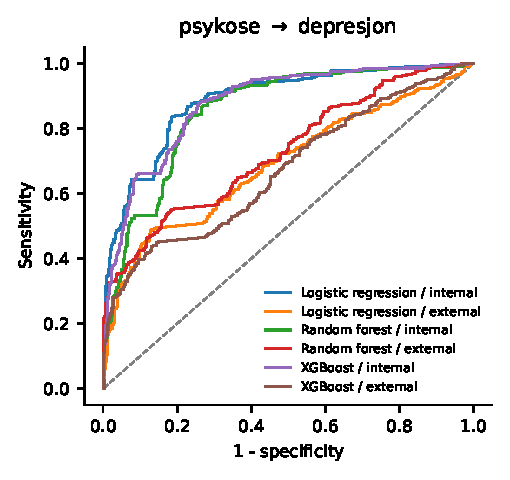
\includegraphics[width=.49\columnwidth]{e2_roc_psykose_to_depresjon.pdf}\hfill
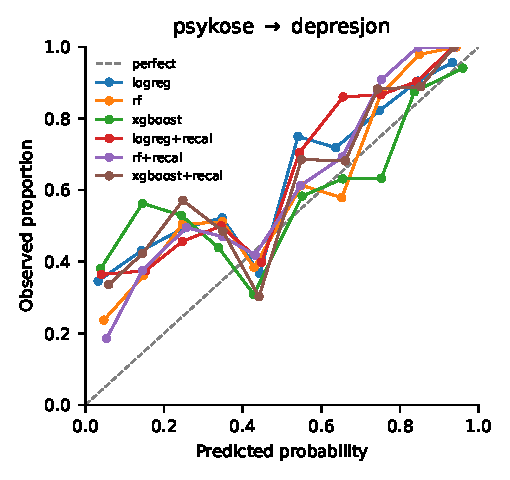
\includegraphics[width=.49\columnwidth]{e3_reliability_psykose_to_depresjon.pdf}
\caption{PSYKOSE$\rightarrow$DEPRESJON. Left: ROC of internal (subject-wise CV on PSYKOSE) and external (frozen model on DEPRESJON) predictions. Right: reliability of the external predictions before and after recalibration fitted on the training cohort.}\label{fig:e2}\end{figure}
Transfer was asymmetric (Table~\ref{tab:e2}). DEPRESJON-trained models separated schizophrenia from the held-out controls as well as they had separated depression internally (external 0.769 to 0.779 versus internal 0.764 to 0.779). PSYKOSE-trained models lost 0.13 to 0.21 AUROC on DEPRESJON (logistic regression 0.885$\rightarrow$0.689; XGBoost 0.877$\rightarrow$0.671) with slopes 0.27 to 0.63, intercepts 0.74 to 1.44 and Brier 0.22 to 0.29 against 0.25 for a constant prediction (Fig.~\ref{fig:e2}). The label-shift pair fell to 0.442 to 0.460. Participant-level events per predictor in the training cohorts were 0.6 to 0.8.

\subsection{E3: calibration}
\begin{figure}[!t]\centering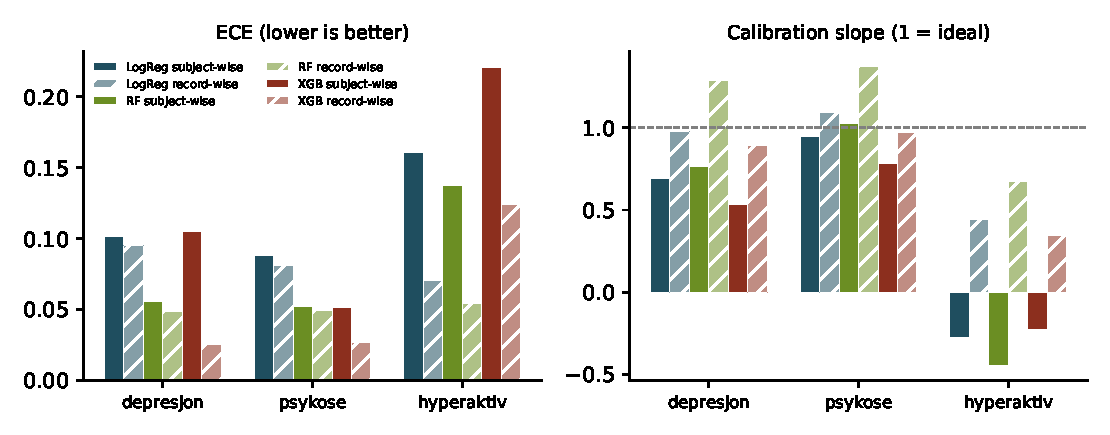
\includegraphics[width=\columnwidth]{e3_ece_slope_comparison.pdf}
\caption{ECE (left) and calibration slope (right) under subject-wise (solid) and record-wise (hatched) cross-validation.}\label{fig:ece}\end{figure}
Under honest splitting the models were already miscalibrated (Fig.~\ref{fig:ece}; full table in Supplementary Table S7): slopes 0.53 to 0.77 on DEPRESJON, 0.95 on PSYKOSE, and negative on HYPERAKTIV with ECE 0.14 to 0.22, i.e.\ confident probabilities from models that had learned nothing. Record-wise models looked \emph{better} calibrated in-sample because they scored participants they had seen. Recalibration on the training cohort repaired the easy transfer direction (DEPRESJON$\rightarrow$PSYKOSE: slopes 1.05, ECE 0.04 to 0.05) but not the hard one (PSYKOSE$\rightarrow$DEPRESJON: slopes 0.35 to 0.77, ECE 0.13 to 0.20), because that miscalibration is a property of the population shift.

\subsection{E5 and E6: transdiagnostic tasks and ablation}
\wideon% placeholder until E5 completes
\wideoff
On OBF-Psychiatric, any psychiatric group versus healthy control reached 0.776 to 0.795 subject-wise and 0.824 to 0.849 record-wise; five-class macro-AUROC was 0.695 to 0.713 versus 0.770 to 0.811 (Table~\ref{tab:e5}). Under subject-wise CV, dropping any feature group, applying SMOTE inside folds, or replacing five-fold with leave-one-subject-out changed AUROC by at most 0.06 and no variant on HYPERAKTIV rose above chance (Supplementary Table S8): the gap between published and honest numbers is a property of the splitting design, not of feature engineering.

\section{Published claims against the measured bands}\label{sec:claims}
\wideon%% J-BHI copy of ../empirical/tables/sota_comparison.tex: caption points to Supplementary Table S4
%% (the study list is in the separately compiled supplement, so \ref{tab:part1} cannot resolve here).
% Auto-generated by scripts/part2_extra_figures.py
\begin{table}[!htbp]\centering\caption{Published best accuracies on each cohort (study IDs as in Supplementary Table S4) against the accuracy and AUROC bands measured in this study under subject-wise and record-wise five-fold cross-validation (window level unless stated; seed-averaged estimates, range over logistic regression, random forest and XGBoost).}\label{tab:sota}\footnotesize
\begin{adjustbox}{max width=\linewidth}
\begin{tabular}{lp{4.2cm}p{1.9cm}p{1.9cm}p{1.9cm}p{1.9cm}p{2.1cm}}
\toprule
Cohort & Published best accuracies (ID value) & Measured accuracy, subject-wise (range over models) & Measured accuracy, record-wise & Measured AUROC, subject-wise & Measured AUROC, record-wise & Measured subject-level AUROC, subject-wise \\
\midrule
DEPRESJON & S02 0.89, S07 0.77, S09 0.78, S10 0.96, S16 0.94, S19 0.85 & 0.72--0.72 & 0.77--0.81 & 0.76--0.78 & 0.84--0.88 & 0.87--0.90 \\
PSYKOSE & S15 0.92, S16 0.94 & 0.86--0.87 & 0.87--0.89 & 0.89--0.91 & 0.93--0.95 & 0.96--0.97 \\
HYPERAKTIV & -- & 0.44--0.46 & 0.53--0.57 & 0.44--0.45 & 0.58--0.61 & 0.42--0.44 \\
\bottomrule
\end{tabular}
\end{adjustbox}\end{table}
\wideoff
\begin{figure*}[!t]\centering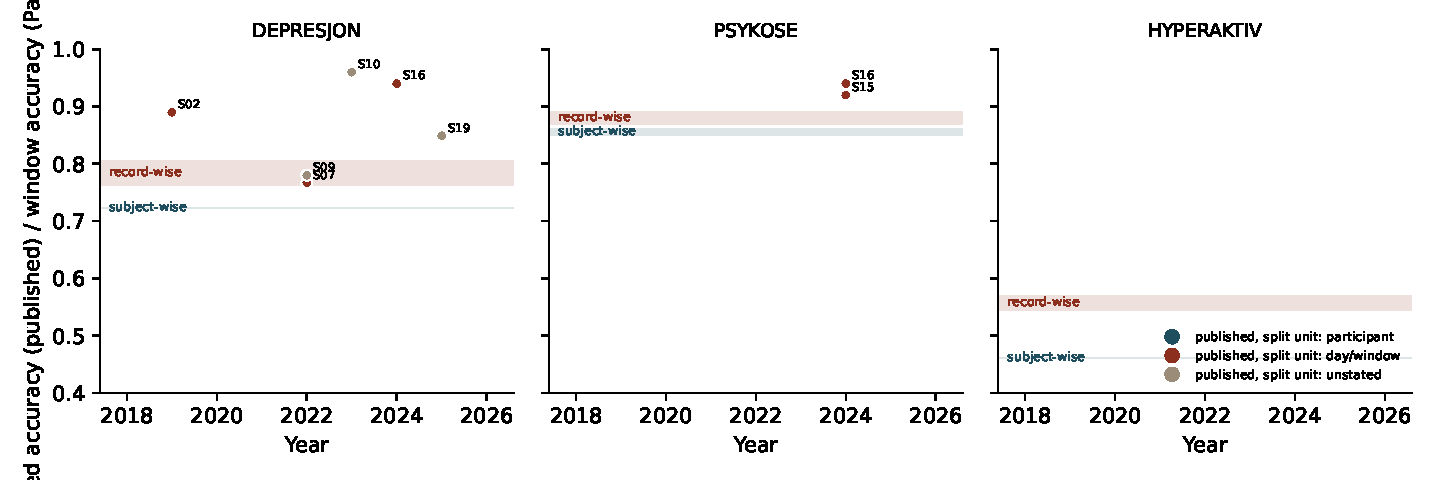
\includegraphics[width=\textwidth]{part1_claims_vs_bands.pdf}
\caption{Published best accuracies (labelled by study ID, Supplementary Table S4; coloured by the unit of splitting) against the window-level accuracy bands measured here under subject-wise and record-wise cross-validation.}\label{fig:part1}\end{figure*}
Twenty-eight published supervised models on the four cohorts were identified by citation tracing of the dataset papers and dataset-name searches (September 2026) and extracted against a fixed codebook for PROBAST+AI and TRIPOD+AI criteria: unit of splitting, external validation, calibration, events per predictor, code availability and handling of the shared controls (Supplementary Tables S3 and S4; 24 extracted from abstract and metadata, marked as such). Seven split by participant, 9 by day, 12 did not state the unit (21 of 28 day-level or unstated, 75\%, Wilson 95\% CI 57 to 87\%); none reported calibration (0 to 12\%); none validated on a second cohort; 4 released code (14\%, 6 to 31\%); none of the four studies combining DEPRESJON and PSYKOSE, other than the OBF descriptor, states how the shared controls were handled. Table~\ref{tab:sota} and Fig.~\ref{fig:part1} place the claims beside the measured bands: every accuracy above the subject-wise band on DEPRESJON (0.89, 0.96, 0.85) lies inside or above the record-wise band and used or did not state a day-level unit; the PSYKOSE claims of 0.92 and 0.94 sit at the top of the record-wise band; for ADHD versus clinical controls the honest band is chance. The numbers reproduce; what they measure is participant identity.

\section{Discussion}
Each practice the appraisal criteria flag changed conclusions on real data, always towards optimism, and the mechanism is now demonstrated rather than argued: record-wise splitting scores 0.69 to 0.90 on labels without any disorder signal, a day of activity identifies its owner with 27 to 40\% top-1 accuracy among up to 80 people, inflation grows with model flexibility, and a state-of-the-art time-series learner reproduces it. The clinically relevant quantities on these data are participant-level AUROC of about 0.87 to 0.90 for depression and 0.96 to 0.97 for schizophrenia against healthy controls, no discrimination for ADHD against other psychiatric outpatients, and probabilities that need recalibration in the target population. The distinction between healthy and clinical controls matters: HYPERAKTIV shows how quickly the actigraphy signal disappears when the comparison becomes realistic.

\emph{Limitations.} One device family and country; small participant numbers with wide participant-level intervals; group labels rather than symptom trajectories; a single window length; fixed rather than tuned models (tuning inside subject-wise folds would raise honest performance somewhat without changing the paired inflation, which is the estimand); no demographic predictors; in E2 a control group split rather than an independent one; the appraisal of published models was identified by citation tracing rather than exhaustive database searches, was not registered, and rests on abstracts for 24 of 28 studies, so an unstated unit may hide participant-level splitting (it was never counted as day-level). We did not reproduce individual published pipelines; a specific architecture could sit above the bands for reasons other than leakage, which its authors can show by reporting subject-wise results.

\section{Conclusion}
For any repeated-measures mental-health dataset: state the unit of splitting; report participant-level as well as window-level sample sizes and metrics; report calibration slope and intercept with a reliability curve; check for shared participants across combined datasets; release code with run manifests. The released protocol enforces the first four by construction and the baselines give future work on these cohorts a reference: a claim above the honest band invites one question, namely which splitting unit produced it.

\section*{Acknowledgment}
The author thanks the custodians of the DEPRESJON, PSYKOSE, HYPERAKTIV and OBF-Psychiatric datasets for making them openly available. Data: \url{https://datasets.simula.no/} and \url{https://zenodo.org/records/13754984}. Code: see the first-page footnote (release v1.0.0-submission).

\begin{thebibliography}{1}
\bibitem{garciaceja2018} E. Garcia-Ceja, M. Riegler, P. Jakobsen \emph{et al.}, ``Depresjon: A motor activity database of depression episodes in unipolar and bipolar patients,'' in \emph{Proc. ACM MMSys}, 2018, doi:10.1145/3204949.3208125.
\bibitem{jakobsen2020} P. Jakobsen, E. Garcia-Ceja, L. A. Stabell \emph{et al.}, ``PSYKOSE: A motor activity database of patients with schizophrenia,'' in \emph{Proc. IEEE CBMS}, 2020, doi:10.1109/CBMS49503.2020.00064.
\bibitem{hicks2021} S. A. Hicks, A. Stautland, O. B. Fasmer \emph{et al.}, ``HYPERAKTIV: An activity dataset from patients with attention-deficit/hyperactivity disorder (ADHD),'' in \emph{Proc. ACM MMSys}, 2021, doi:10.1145/3458305.3478454.
\bibitem{obf2025} E. Garcia-Ceja \emph{et al.}, ``OBF-Psychiatric, a motor activity dataset of patients diagnosed with major depression, schizophrenia, and ADHD,'' \emph{Sci. Data}, vol. 12, 2025, doi:10.1038/s41597-025-04384-3.
\bibitem{jmir2025} ``Explainable AI for depression detection and severity classification from activity data,'' \emph{JMIR Ment. Health}, vol. 12, p. e72038, 2025.
\bibitem{arxiv2303} ``Transfer learning for real-time deployment of a screening tool for depression detection using actigraphy,'' arXiv:2303.07847, 2023.
\bibitem{zanella2019} L. A. Zanella-Calzada \emph{et al.}, ``Feature extraction in motor activity signal: Towards a depression episodes detection in unipolar and bipolar patients,'' \emph{Diagnostics}, vol. 9, no. 8, 2019.
\bibitem{psykose_dl2024} ``Objective diagnosis of psychotic disorders using multi-branch deep learning on time-series motor activity signals,'' \emph{Soft Comput.}, 2024, doi:10.1007/s00500-024-09832-7.
\bibitem{psykose_bspc2024} ``Unveiling psychotic disorder patterns: A deep learning model analysing motor activity time-series data with explainable AI,'' \emph{Biomed. Signal Process. Control}, 2024.
\bibitem{saeb2017} S. Saeb, L. Lonini, A. Jayaraman, D. C. Mohr, and K. P. Kording, ``The need to approximate the use-case in clinical machine learning,'' \emph{GigaScience}, vol. 6, no. 5, p. gix019, 2017.
\bibitem{jmirai2026} A. Karbalaie, F. Abtahi, and C. H\"ager, ``Participant-aware model validation for repeated-measures data: Comparative cross-validation study,'' \emph{JMIR AI}, vol. 5, p. e87728, 2026.
\bibitem{vancalster2019} B. Van Calster, D. J. McLernon, M. van Smeden \emph{et al.}, ``Calibration: The Achilles heel of predictive analytics,'' \emph{BMC Med.}, vol. 17, p. 230, 2019.
\bibitem{moons2025} K. G. M. Moons, J. A. A. Damen, T. Nair \emph{et al.}, ``PROBAST+AI: An updated quality, risk of bias, and applicability assessment tool for prediction models using regression or artificial intelligence methods,'' \emph{BMJ}, vol. 388, p. e082505, 2025.
\bibitem{collins2024} G. S. Collins, K. G. M. Moons, P. Dhiman \emph{et al.}, ``TRIPOD+AI statement: Updated guidance for reporting clinical prediction models that use regression or machine learning methods,'' \emph{BMJ}, vol. 385, p. e078378, 2024.
\bibitem{meehan2022} A. J. Meehan, S. J. Lewis, S. Fazel \emph{et al.}, ``Clinical prediction models in psychiatry: A systematic review of two decades of progress and challenges,'' \emph{Mol. Psychiatry}, vol. 27, pp. 2700--2708, 2022.
\bibitem{dempster2020} A. Dempster, F. Petitjean, and G. I. Webb, ``ROCKET: Exceptionally fast and accurate time series classification using random convolutional kernels,'' \emph{Data Min. Knowl. Discov.}, vol. 34, pp. 1454--1495, 2020.
\end{thebibliography}
\end{document}
